\documentclass{beamer}

\usepackage{algorithm}
\usepackage{algpseudocode}
\usepackage{amsfonts,amsbsy,amsthm,amsmath,amssymb}
\usepackage{beamerthemesplit}
\usepackage{comment}
\usepackage{listings}
\usepackage{multirow}

\DeclareMathOperator*{\argmax}{arg\,max}
\DeclareMathOperator*{\argmin}{arg\,min}
\DeclareMathOperator{\ord}{ord}
\DeclareMathOperator{\sign}{sign}

\algtext*{EndWhile}      % Remove "end while" text
\algtext*{EndIf}         % Remove "end if" text
\algtext*{EndFor}        % Remove "end for" text
\algtext*{EndProcedure}  % Remove "end procedure" text
\renewcommand{\algorithmiccomment}[1]{\hfill \{#1\}}
\renewcommand{\algorithmicrequire}{\textbf{Input:}}
\renewcommand{\algorithmicensure}{\textbf{Output:}}
\newcommand{\algnewline}{\par\noindent\hskip\algorithmicindent}

\newcommand{\CC}{\mathbb{C}}
\newcommand{\NN}{\mathbb{N}}
\newcommand{\RR}{\mathbb{R}}
\newcommand{\ZZ}{\mathbb{Z}}
\newcommand{\QQ}{\mathbb{Q}}
\newcommand{\RRgtz}{\mathbb{R}_{>0}}
\newcommand{\ZZgtz}{\mathbb{Z}_{>0}}
\newcommand{\ZZgez}{\mathbb{Z}_{\ge 0}}
\newcommand{\QQgtz}{\mathbb{Q}_{>0}}
\newcommand{\QQgez}{\mathbb{Q}_{\ge 0}}

\newcommand{\KK}{\mathcal{K}}
\newcommand{\MM}{\mathcal{M}}
\newcommand{\OO}{\mathcal{O}}

\newcommand{\matrixto}[2]{\left[ \begin{array}{rr} #1 & #2 \end{array} \right]}
\newcommand{\matrixot}[2]{\left[ \begin{array}{r} #1 \\ #2 \end{array} \right]}
\newcommand{\matrixtt}[4]{\left[ \begin{array}{rr} #1 & #2 \\ #3 & #4 \end{array} \right]}
\newcommand{\matrixltt}[4]{\left[ \begin{array}{ll} #1 & #2 \\ #3 & #4 \end{array} \right]}
\newcommand{\matrixThreeOne}[3]{\left[ \begin{array}{rrr} #1 & #2 & #3 \end{array} \right]}
\newcommand{\matrixThreeTwo}[6]{\left[ \begin{array}{rrr} #1 & #2 & #3 \\ #4 & #5 & #6 \end{array} \right]}
\newcommand{\ntoinfty}{\lim_{n \rightarrow \infty}}
\newcommand{\floor}[1]{\left\lfloor #1 \right\rfloor}
\newcommand{\ceil}[1]{\left\lceil #1 \right\rceil}

\newcommand{\band}{~\texttt{and}_\texttt{2}~}
\newcommand{\bor}{~\texttt{or}_\texttt{2}~}
\newcommand{\bxor}{\oplus}
\newcommand{\bnot}{\lnot}
\newcommand{\binary}[1]{\texttt{#1}_\texttt{2}}

\newcommand{\set}{\mathcal}
\newcommand{\ideal}{\mathfrak}
\newcommand{\idealclass}[1]{\left[ \ideal #1 \right]}
\newcommand{\aclass}{\idealclass a}
\newcommand{\bclass}{\idealclass b}
\newcommand{\cclass}{\idealclass c}
\newcommand{\dclass}{\idealclass d}
\newcommand{\pclass}{\idealclass p}
\newcommand{\qclass}{\idealclass q}
\newcommand{\idclass}{[\mathcal O_\Delta]}

\newcommand{\ith}{i^{\textrm{th}}}

\newcommand{\smallfont}{\fontsize{6pt}{7.2}\selectfont}

\graphicspath{{eps/}{png/}{l2r-best-approx/}}

\title[]{Improved Arithmetic in the Ideal Class Group of Imaginary Quadratic Number Fields}
\subtitle{With an Application to Integer Factoring}
\author{Maxwell Sayles}
\date{May 22, 2013}
\institute{
	\bigskip 
       Department of Computer Science \\
       University of Calgary
}

\usetheme{Copenhagen}
\setbeamertemplate{navigation symbols}{} %no nav symbols

% TODO: Force page count
\makeatletter
\setbeamertemplate{footline}
{%
  \leavevmode%
  \hbox{\begin{beamercolorbox}[wd=.5\paperwidth,ht=2.5ex,dp=1.125ex,leftskip=.3cm plus1fill,rightskip=.3cm]{author in head/foot}%
    \usebeamerfont{author in head/foot} \hspace*{2em} \insertshortauthor \hspace*{2em}
  \end{beamercolorbox}%
  \begin{beamercolorbox}[wd=.5\paperwidth,ht=2.5ex,dp=1.125ex,leftskip=.3cm,rightskip=.3cm plus1fil]{title in head/foot}%
    \usebeamerfont{title in head/foot} \hspace*{2em} \insertframenumber ~/ \inserttotalframenumber \hspace*{2em}
%    \usebeamerfont{title in head/foot} \hspace*{2em} \insertshorttitle \hspace*{2em} \insertframenumber ~/ \inserttotalframenumber \hspace*{2em}
  \end{beamercolorbox}}%
  \vskip0pt%
}
\makeatother


% What's important is to state and motivate the topic, highlight/outline your original results and contributions, give an overview of your methodology, assess significance, and give some interesting future work.  

%Ideal Class Group - NUCOMP, NUDUPL, NUCUBE... XGCD
%Exponentiation - 2,3 number system. L2R and Tree based.
%SPAR

%Improvements:
%- XGCD
%- left-to-right best approximations
%- SuperSPAR


\begin{document}
\maketitle

% OVERVIEW
\begin{frame}
\frametitle{Overview}

Major goals:
\begin{itemize}
\item Improve the performance of arithmetic in the ideal class group of imaginary quadratic number fields.
	\begin{itemize}
	\item Specifically when the discriminant of the class group is smaller than 128-bits.
	\end{itemize}
\item An optimized implementation of the SuperSPAR integer factoring algorithm for integers smaller than 128-bits.
\end{itemize}

\end{frame}

% SOME USES
\begin{frame}
\frametitle{Some Possible Applications}
These are just a few possible applications. \bigskip

Ideal class group:
\begin{itemize}
\item Class group tabulation for larger discriminants \break (Ramachandran2006).
\end{itemize}

\bigskip
Integer Factoring:
\begin{itemize}
\item Factoring left-overs after sieving in algorithms like the number field sieve using multiple large primes.
\end{itemize}

\end{frame}

% CONTRIBUTIONS TO IDEAL CLASS GROUP ARITHMETIC
\begin{frame}
\frametitle{Contributions}
Contributions to ideal class group arithmetic:
\begin{itemize} %[<+->]
\item Optimized implementations using 64 and 128-bit arithmetic.
\item Optimized XGCD for 32, 64, and 128-bits.
\end{itemize}

\bigskip
Contributions to integer factoring:
\begin{itemize}
\item Left-to-right best approximations method for computing 2,3 representations of power primorials.
\item SuperSPAR integer factoring algorithm.
\end{itemize}
\end{frame}

% CONTRIBUTIONS TO INTEGER FACTORING
\begin{frame}
\frametitle{Contributions Continued}
Contributions to integer factoring:

\begin{itemize}
\item Left-to-right best approximations method for computing 2,3 representations.
	\begin{itemize}
	\item Tested using power primorials.
	\item Best representations for exponentiation of the methods tested.
	\item Exponentiation is about 1.4 times faster on average than with the binary representations.
		\begin{itemize}
		\item Representations are computed in advance.
		\end{itemize}
	\end{itemize}
\item SuperSPAR integer factoring algorithm.
	\begin{itemize}
	\item Extends SPAR using bounded primorial steps search.
	\item Uses improvements to ideal class group arithmetic and 2,3 representations of power primorials.
	\item On average, fastest integer factoring algorithm for integers of size 50-bits to 62-bits of the implementations tested.
	\end{itemize}
\end{itemize}
\end{frame}
  
% IDEAL CLASS GROUP ARITHMETIC
\begin{frame}
\frametitle{Arithmetic in the Ideal Class Group}
Our implementation is based on NUCOMP, NUDUPL, and NUCUBE. % TODO CITE

\begin{itemize}
\item Implementations for 64-bit and 128-bit arithmetic.
	\begin{itemize}
	\item A reference implementation using GMP.
	\end{itemize}
\item Extended greatest common divisor.
\item Partial extended greatest common divisor.
	\begin{itemize}
	\item Termination bound is approximated using a square root approximation.
	\end{itemize}
\end{itemize}

\end{frame}  

% XGCD
\begin{comment}
\begin{frame}
\frametitle{Extended Greatest Common Divisor (XGCD)}
Extended greatest common divisor solves
\[
	s = Ua + Vb = \gcd(a, b).
\]
Partial extended greatest common divisor solves
TODO: This is madness
\begin{eqnarray*}
	s &= (-1)^z Ua + (-1)^{z+1} Vb \\
	t &= (-1)^z Xa + (-1)^{z+1} Yb
\end{eqnarray*}
for $t \le B < s$ for some termination bound $B$ given by NUCOMP, NUDUPL, or NUCUBE.

\end{frame}
\end{comment}

% XGCD Experiments
\begin{frame}
\frametitle{XGCD Experiments}
\begin{itemize}
\item 32-bit, 64-bit, 128-bit implementations.
\item Extended Euclidean Algorithm.
\item Windowed right-to-left binary XGCDs (Stein).
\item Left-to-right binary XGCDs (Shallit and Sorenson, Brent${}^{*}$, and our simplified).
\item Lehmer's XGCD (8-bit precomputed, 32-bit EEA, 64-bit EEA and L2R).
\item Pari, GMP, and Flint${}^{*}$ as reference implementations.
\item 1,000,000 pseudorandom positive integer pairs $(a,b)$ for each bit size.
\end{itemize}

\smallfont
Items marked with ${}^{*}$ did not appear in thesis.
\end{frame}

% BRENT'S XGCD
\begin{frame}
\frametitle{Brent's Left-to-Right Binary XGCD}
\begin{algorithmic}[1]
\Procedure{BrentXGCD}{$a, b}$ \Comment{$a, b \in \ZZgez$}
\State $\matrixThreeTwo{s}{U}{V}{t}{X}{Y} \gets \matrixThreeTwo{a}{1}{0}{b}{0}{1}$
\While {$t > 0$}
	\State find the largest $k$ such that $2^k t \le s$
	\State $\matrixThreeTwo{s}{U}{V}{t}{X}{Y} \gets \matrixtt{1}{-2^k}{0}{1} \cdot
		    \matrixThreeTwo{s}{U}{V}{t}{X}{Y}$
	\If {$s < t$} swap the rows of the matrix \EndIf
\EndWhile
\State \Return $(s, U, V)$
\EndProcedure
\end{algorithmic}
\end{frame}

% LEFT-TO-RIGHT BINARY XGCDs
\begin{frame}
\frametitle{Left-to-Right Binary XGCDs}
\framesubtitle{32-bit}
\begin{figure}
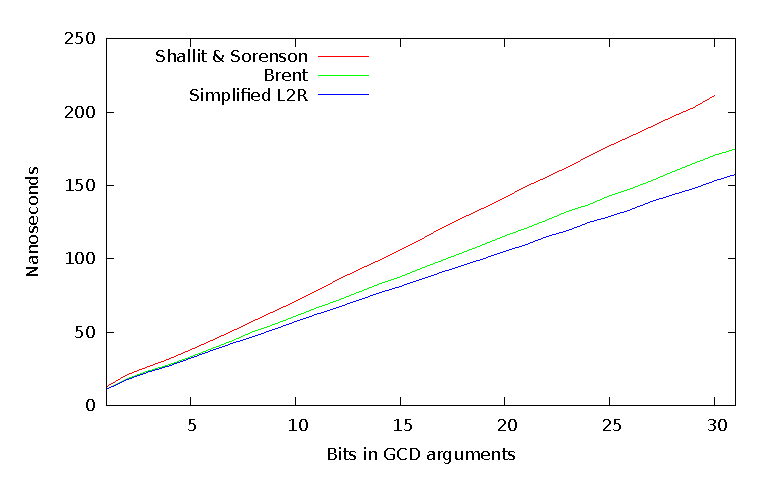
\includegraphics[scale=0.86]{xgcds-binary-32}
\end{figure}
\end{frame}
\begin{frame}
\frametitle{Left-to-Right Binary XGCDs}
\framesubtitle{64-bit}
\begin{figure}
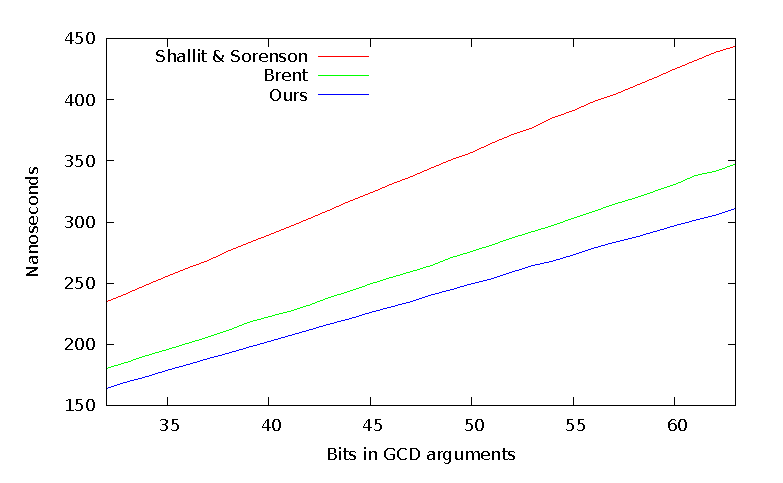
\includegraphics[scale=0.86]{xgcds-binary-64}
\end{figure}
\end{frame}
\begin{frame}
\frametitle{Left-to-Right Binary XGCDs}
\framesubtitle{128-bit}
\begin{figure}
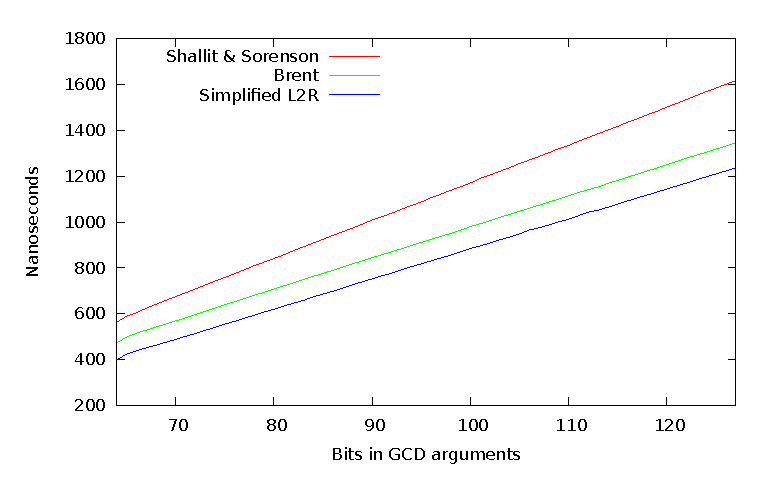
\includegraphics[scale=0.86]{xgcds-binary-128}
\end{figure}
\end{frame}

% XGCD Results
\begin{frame}
\frametitle{XGCD Results}
\framesubtitle{32-bit}
\begin{figure}
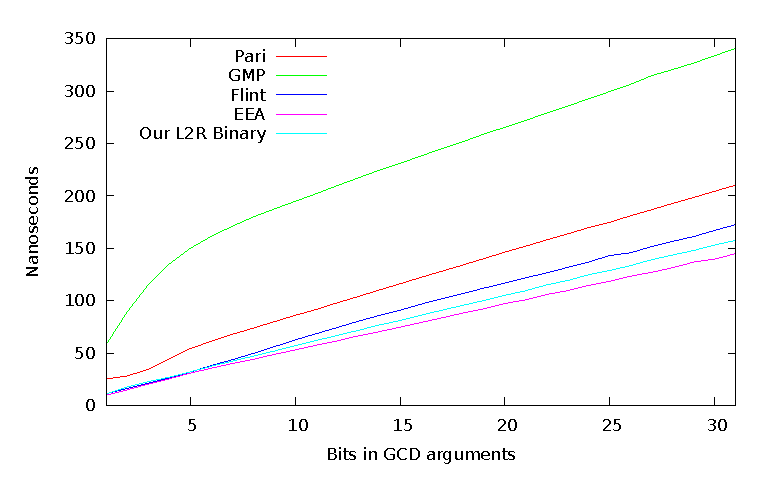
\includegraphics[scale=0.86]{xgcd-best-32}
\end{figure}
\end{frame}
\begin{frame}
\frametitle{XGCD Results}
\framesubtitle{64-bit}
\begin{figure}
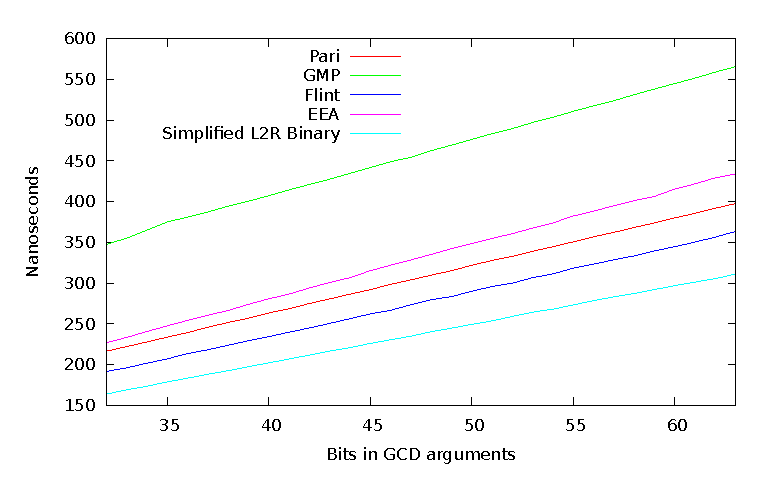
\includegraphics[scale=0.86]{xgcd-best-64}
\end{figure}
\end{frame}
\begin{frame}
\frametitle{XGCD Results}
\framesubtitle{128-bit}
\begin{figure}
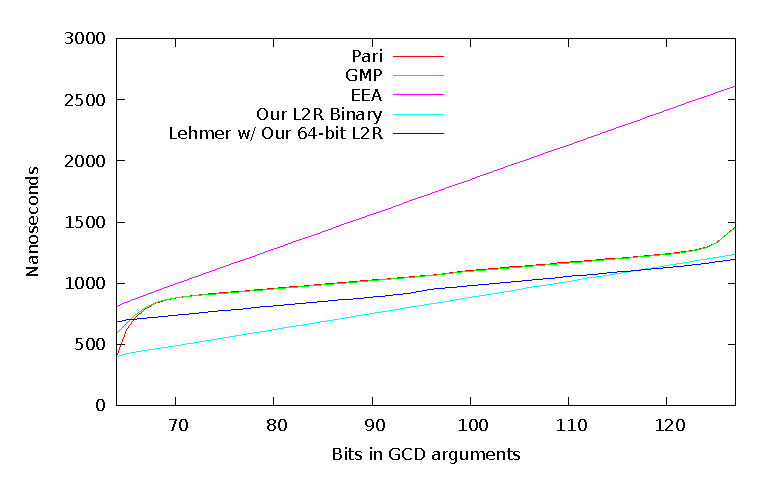
\includegraphics[scale=0.86]{xgcd-best-128}
\end{figure}
\end{frame}

% XGCD QUANTIFIED RESULTS
\begin{frame}
\frametitle{XGCD Improvement}

How much faster than the reference implementations?
\begin{table}
\centering
\begin{tabular}{ | r | l | r | r | r | }
\hline
Bit Range & Algorithm & GMP & Pari & Flint \\
\hline
1 -- 31 & EEA & 3.44 & 1.60 & 1.17 \\
32 -- 63 & Simplified L2R Binary & 1.94 & 1.29 & 1.16 \\
64 -- 118 & Simplified L2R Binary & 1.38 & 1.38 & -- \\
119 -- 127 & Lehmer w/ 64-bit Simplified & 1.12 & 1.13 & -- \\
\hline
\end{tabular}
\end{table}

\bigskip
\smallfont
All times are based on the average.  The measurement of improvement is an average over the bit range.
\end{frame}

% Partial XGCD Experiments
\begin{frame}
\frametitle{Partial XGCD Experiments}
Operations of XGCD must be unimodular.
%Operations of XGCD must be unimodular and partial quotients are terms in a simple continued fraction expansion\footnote{Results are not in thesis.}.
\begin{itemize}
\item 32-bit, 64-bit, 128-bit implementations.
\item Extended Euclidean Algorithm.
\item Left-to-right binary XGCD (Brent).
\item Lehmer's XGCD (8-bit precomputed, 32-bit EEA, 64-bit EEA and L2R).
\item 1,000,000 pseudorandom positive integer triples $(a, b, T)$ with $0 \le b \le a$ and $0 \le T \le \sqrt a$.
\end{itemize}

\bigskip
\smallfont
Results are not in thesis.
\end{frame}

% PARTIAL XGCD RESULTS
\begin{frame}
\frametitle{Partial XGCD Results}
\framesubtitle{32-bits}
\begin{figure}
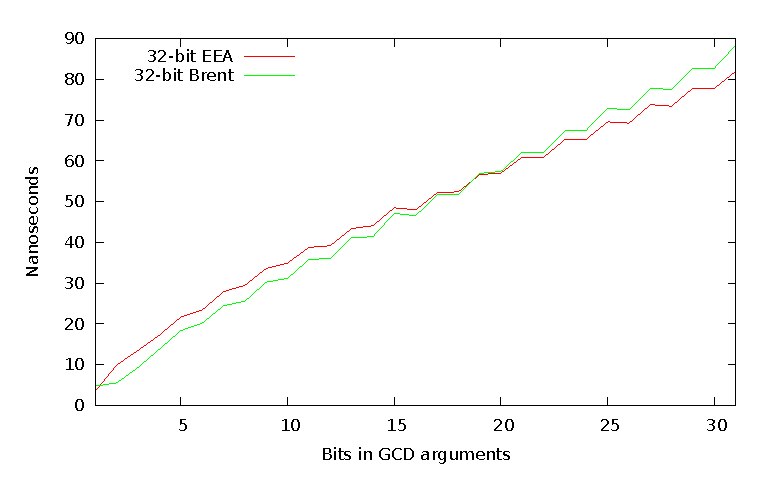
\includegraphics[scale=0.86]{best-partial-32}
\end{figure}
\end{frame}
\begin{frame}
\frametitle{Partial XGCD Results}
\framesubtitle{64-bits}
\begin{figure}
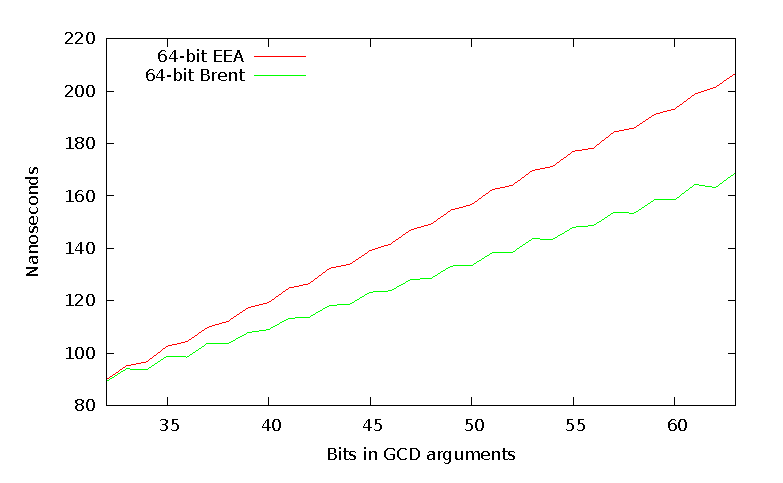
\includegraphics[scale=0.86]{best-partial-64}
\end{figure}
\end{frame}
\begin{frame}
\frametitle{Partial XGCD Results}
\framesubtitle{128-bits}
\begin{figure}
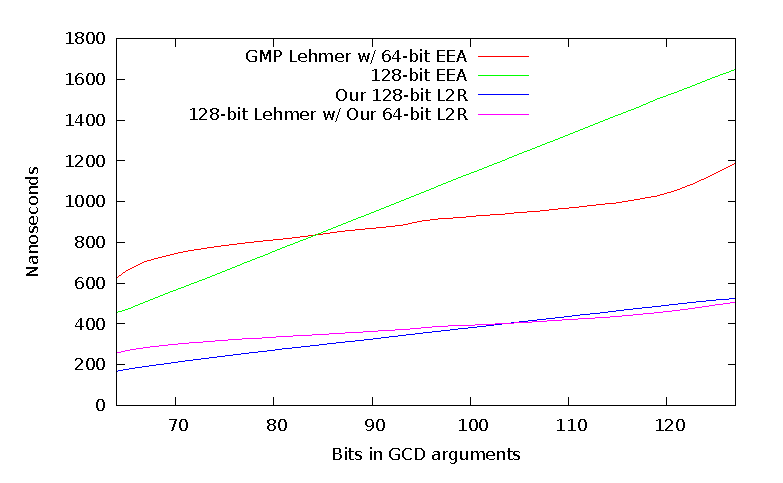
\includegraphics[scale=0.86]{best-partial-128}
\end{figure}
\end{frame}

% PXGCD QUANTIFIED RESULTS
\begin{frame}
\frametitle{Partial XGCD Improvement}
How much faster than the reference implementation?
\begin{table}
\centering
\begin{tabular}{ | r | l | r | }
\hline
\multirow{2}{*}{Bit Range} & \multirow{2}{*}{Algorithm} & GMP Lehmer \\
& & w/ 64-bit EEA \\
\hline
1 -- 18 & Brent & 10.62 \\
19 -- 31 & EEA & 5.95 \\
32 -- 63 & Brent & 4.03 \\
64 -- 88 & Brent & 2.75 \\
89 -- 127 & Lehmer w/ 64-bit Brent & 2.15 \\
\hline
\end{tabular}
\end{table}

\bigskip
\smallfont
All times are based on the average.  The measurement of improvement is an average over the bit range.

\end{frame}



% IDEAL CLASS GROUP EXPERIMENTS
\begin{frame}
\frametitle{Ideal Class Group Experiments}
TODO: Took about a day
\end{frame}

% IDEAL CLASS GROUP RESULTS
\begin{frame}
\frametitle{Ideal Class Group Results}
TODO: insert pretty picture
	\begin{itemize}
	\item 3 to 4 times faster on average than Pari.
	\end{itemize}
\end{frame}

% SPAR/SUPERSPAR
\begin{frame}
\frametitle{SPAR/SuperSPAR}
Two stages:
\begin{itemize}
\item Exponentiate a random ideal class.
\item Search for the order of the resulting ideal class.
\end{itemize}
\end{frame}

% EXPONENTIATION
\begin{frame}
\frametitle{Exponentiation by Odd Power Primorials}
The goal is to compute
\[
\aclass ^ E
\]
for some ideal class $\aclass$ and exponent
\[
	E = \prod_{i=2}^k {p_i}^{e_i}
\]
where $p_i$ is the $\ith$ prime.
\end{frame}

% EXPONENTIATION METHODS
\begin{frame}
\frametitle{Representations Tested}
Representations Tested:
\begin{itemize}
\item Binary, Non-Adjacent Form.
\item Right-to-Left and $2^2 3^2$ Windowed Right-to-Left (Ciet et al.).
\item Left-to-Right (Berth{\'e} and Imbert)
\end{itemize}
\end{frame}

% L2R BEST APPROXIMATIONS
\begin{frame}
\frametitle{Left-to-Right Best Approximations}
Left-to-Right best approximations is a technique combining the greedy approach of Berth{\'e} and Imbert with the tree based approach of Doche and Habsieger.
\begin{itemize}
\item Iterate on a set of partial representations $x + \sum s_i2^{a_i}3^{b_i}$.
\item Keep the best $2^a 3^b$ approximations for each $x$.
\item Squares and cubes are bound $a \le A$, $b \le B$, and the bounds $A$ and $B$ are iterated.
\end{itemize}
\end{frame}

\begin{frame}
\frametitle{Left-to-Right Best Approximations}
\framesubtitle{Example -- First Iteration on 777}
\begin{figure}
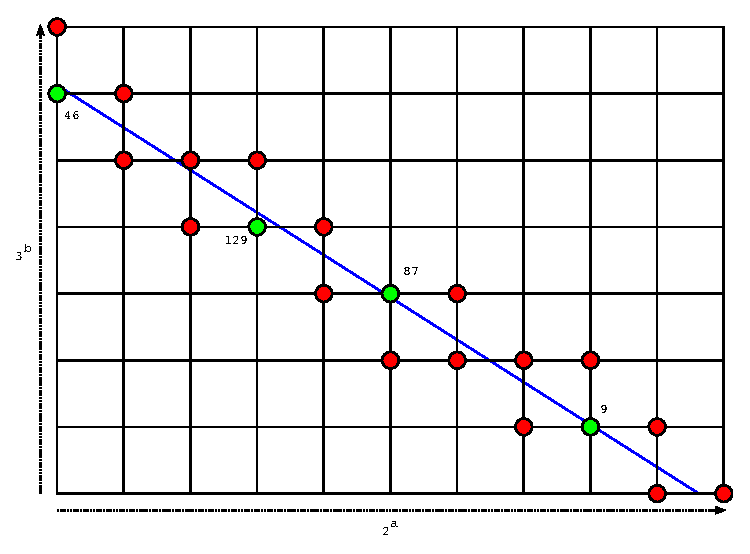
\includegraphics[scale=0.84]{best-approx-777}
\end{figure}
\end{frame}
\begin{frame}
\frametitle{Left-to-Right Best Approximations}
\framesubtitle{Example -- Second Iteration on 9, 48, 87, and 129}
\begin{figure}
\includegraphics[scale=0.84]{best-approx-9-48-87-129}
\end{figure}
\end{frame}
\begin{frame}
\frametitle{Left-to-Right Best Approximations}
\framesubtitle{Example Results}
2,3 Representations for $E=777$:
\begin{align*}
2^8 3^1 + 2^0 3^2 && \textrm{8 squares, 2 cubes, 1 multiplication} \\
2^0 3^6 + 2^4 3^1 && \textrm{4 squares, 6 cubes, 1 multiplication} \\
2^8 3^1 + 2^3 3^0 + 2^0 3^0 && \textrm{8 squares, 1 cube, 2 multiplications} \\
2^3 3^4 + 2^7 3^0 + 2^0 3^0 && \textrm{7 squares, 4 cubes, 2 multiplications}
\end{align*}

\bigskip
$2^8 3^1 + 2^3 3^0 + 2^0 3^0$ possibly preferred since multiplication is cheaper than squaring.
\end{frame}

% EXPONENTIATION EXPERIMENTS
\begin{frame}
\frametitle{Exponentiation Experiments}
TODO: Use results of ideal class group arithmetic experiments to estimate the cost of each
\begin{itemize}
\item Faster.  Each time we change XGCD, we re-time arithmetic, not necessary to retime exponentiation.
\end{itemize}
\end{frame}

% EXPONENTIATION RESULTS (64)
\begin{frame}
\frametitle{Exponentiation Results (64-bit Implementation)}

\begin{figure}
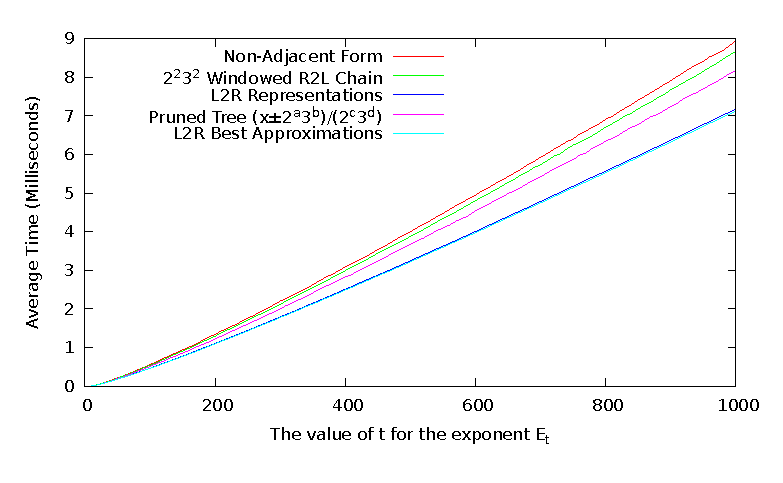
\includegraphics[scale=0.86]{pow-winners-64}
\end{figure}

\end{frame}

% EXPONENTIATION RESULTS (128)
\begin{frame}
\frametitle{Exponentiation Results (128-bit Implementation)}

\begin{figure}
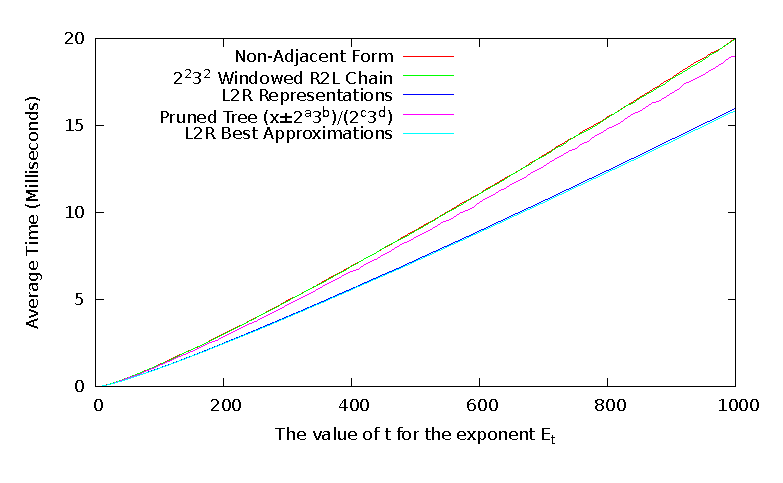
\includegraphics[scale=0.86]{pow-winners-128}
\end{figure}

\end{frame}

% SUPERSPAR
\begin{frame}
\frametitle{SuperSPAR}

SuperSPAR is an integer factoring algorithm based on arithmetic in the ideal class group of imaginary quadratic integers.
\begin{itemize}
\item Extension of SPAR 
\end{itemize}

\end{frame}

% EVOLUTION OF SUPERSPAR
\begin{frame}
\frametitle{Vanilla SPAR}
\begin{figure}
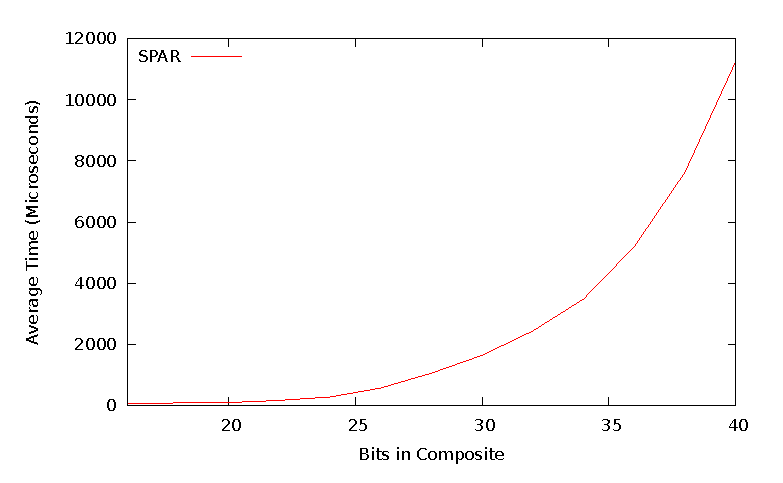
\includegraphics[scale=0.86]{spar-vanilla}
\end{figure}
\end{frame}
\begin{frame}
\frametitle{Bound the Number of Ideals per Group}
\begin{figure}
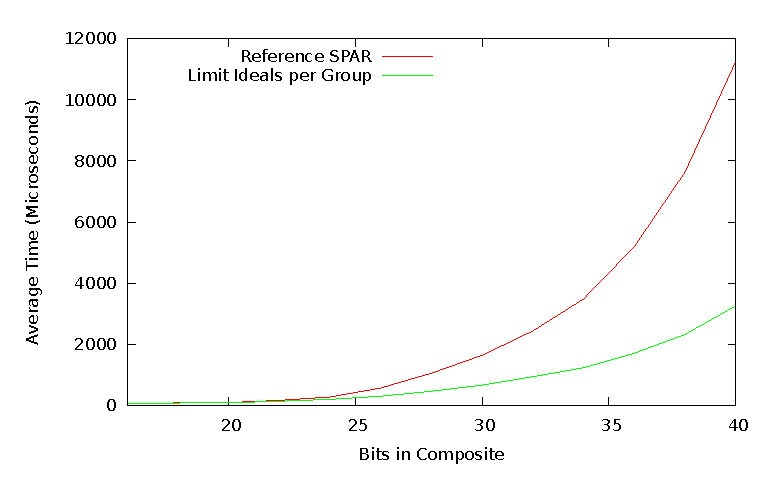
\includegraphics[scale=0.86]{spar-bound-attempts}
\end{figure}
\end{frame}
\begin{frame}
\frametitle{Bound the Number of Ideals per Group}
\begin{figure}
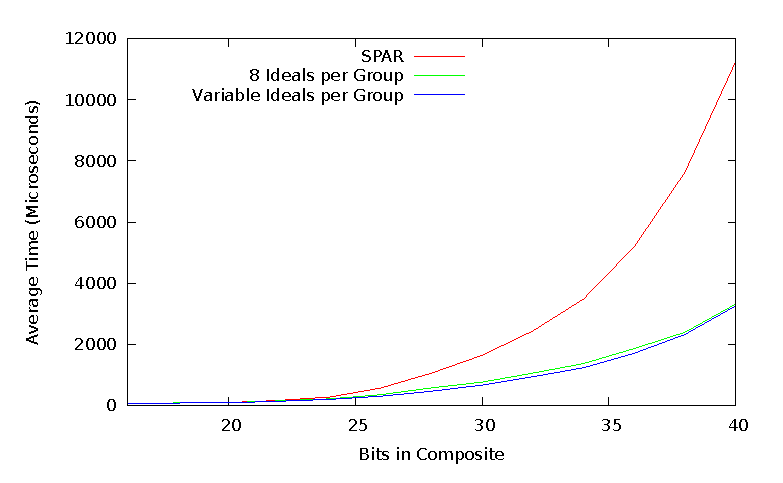
\includegraphics[scale=0.86]{spar-bound-attempts2}
\end{figure}
\end{frame}
\begin{frame}
\frametitle{Bounded Primorial Steps Search}
\begin{figure}
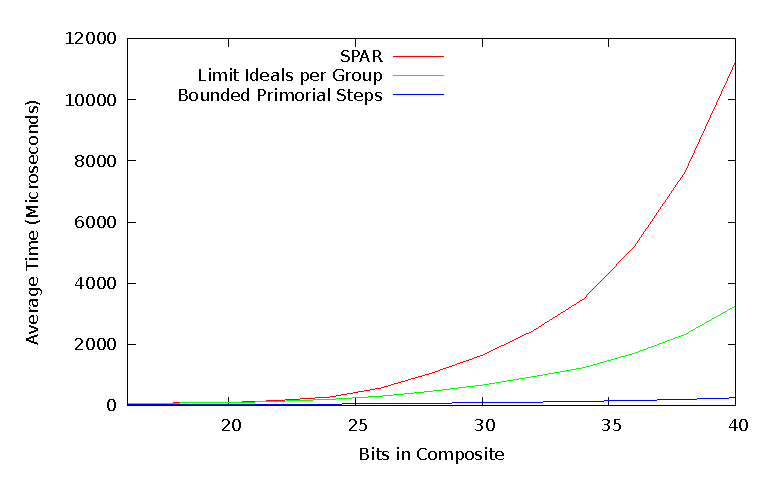
\includegraphics[scale=0.86]{spar-to-sspar}
\end{figure}
\end{frame}
\begin{frame}
\frametitle{Bounded Primorial Steps Search}
\begin{figure}
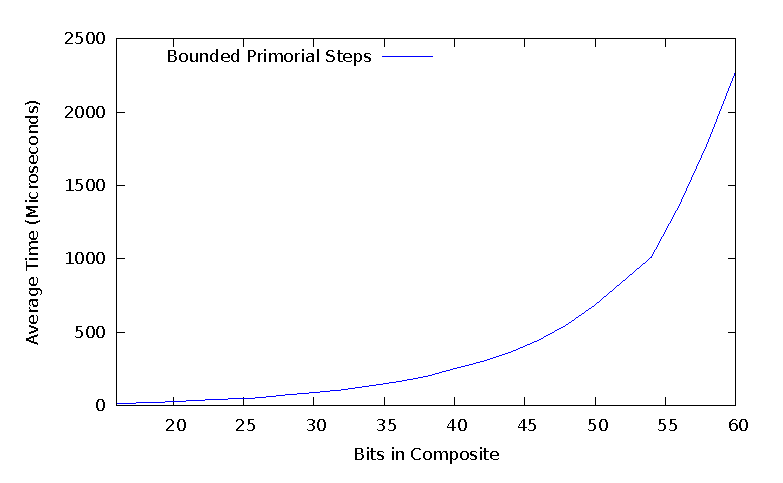
\includegraphics[scale=0.86]{sspar-theoretical}
\end{figure}
\end{frame}
\begin{frame}
\frametitle{Bound $e_i$ in Exponent $E = \prod {p_i}^{e_i}$}
\begin{figure}
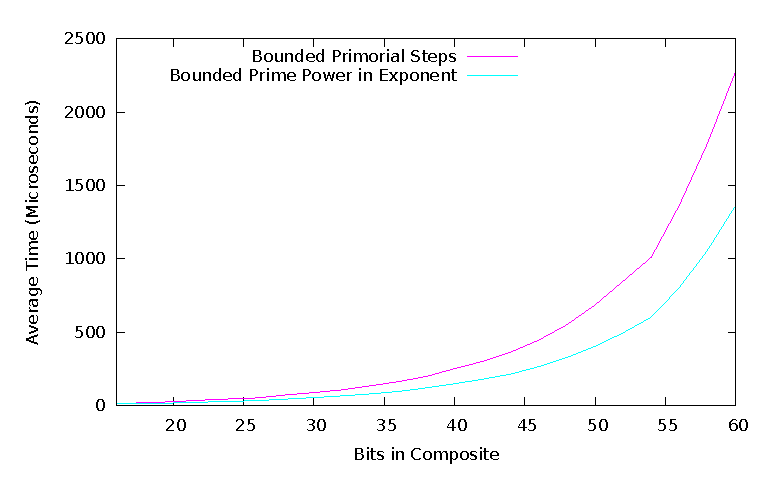
\includegraphics[scale=0.86]{sspar-power-bound}
\end{figure}
\end{frame}
\begin{frame}
\frametitle{Independent Exponent $E$ and Search Bound $mP_w$}
\begin{figure}
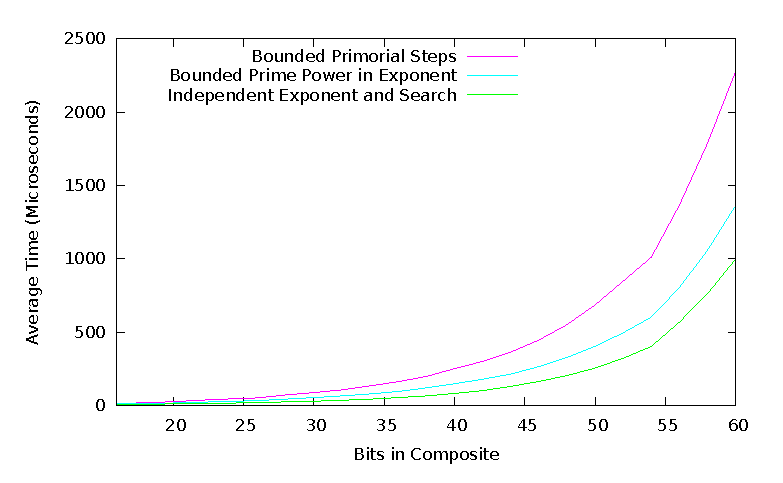
\includegraphics[scale=0.86]{sspar-noreuse}
\end{figure}
\end{frame}
\begin{frame}
\frametitle{Perform a Single Search}
\begin{figure}
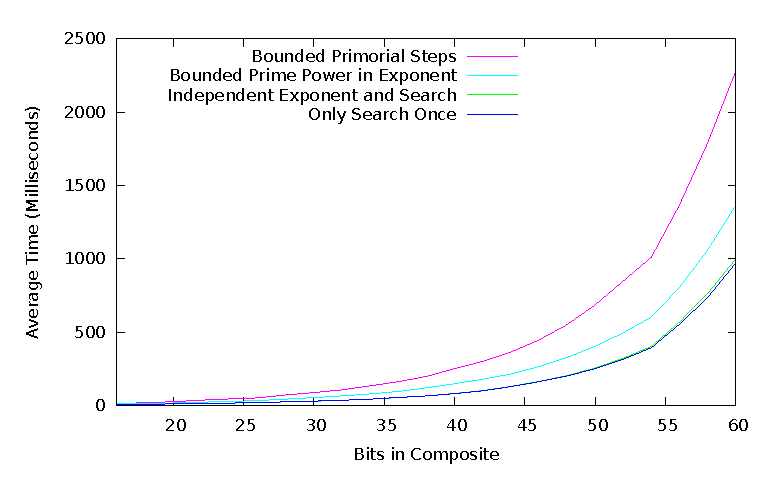
\includegraphics[scale=0.86]{sspar-optimized}
\end{figure}
\end{frame}
\begin{frame}
\frametitle{SPAR vs SuperSPAR}
\begin{figure}
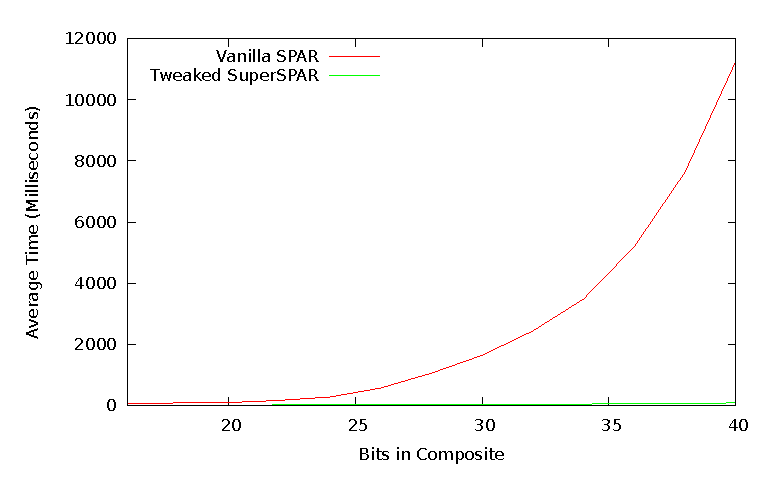
\includegraphics[scale=0.86]{spar-vs-sspar}
\end{figure}
\end{frame}


% FUTURE WORK
\begin{frame}
\frametitle{Future Work}
Some work that is currently in progress or eagerly awaiting:
\begin{itemize}
\item Special case for quotients $q \le 4$ in XGCD.
\item Simplified left-to-right binary partial XGCD.
\item Real quadratic fields and hyperelliptic curves.
\item Improvements to left-to-right best approximations algorithm.
\end{itemize}
\end{frame}

% THANK YOU
\begin{frame}
\frametitle{Thank You}
Summary of performance improvements:
\begin{itemize}
\item Arithmetic in the ideal class group of imaginary quadratic number fields for negative discriminants smaller than 118-bits.
\item The extended GCD for inputs smaller than 128-bits.
\item 2,3 representations for exponentiating by power primorials.
\item Integer factoring for integers 50-bits to 62-bits of size.
\end{itemize}
\end{frame}


%%%%%%%%%%%%%%%%%%
% END OF DEFENCE %
%%%%%%%%%%%%%%%%%%

% FACTORIZATION OF THE ORDER
\begin{frame}
\frametitle{Factorization of the Order}
\framesubtitle{Example \#1}

$N = 9223375433619660527, k = 1, \Delta = -kN$
\begin{itemize}
\item $\ord(\idealclass{p_{19}}) = 2^2 \cdot 13 \cdot 2770667$
\item $\ord(\idealclass{p_{37}}) = 2^3 \cdot 3 \cdot 13 \cdot 2770667$
\item $\ord(\idealclass{p_{43}}) = 2^4 \cdot 3 \cdot 13 \cdot 2770667$
\item $\ord(\idealclass{p_{47}}) = 2^3 \cdot 3 \cdot 13 \cdot 2770667$
\item $\ord(\idealclass{p_{59}}) = 2^4 \cdot 3 \cdot 13 \cdot 2770667$
\end{itemize}

where $\ideal p_p = [p, (b + \sqrt\Delta)/2]$.

\bigskip
Each prime ideal split $N$.

\end{frame}

\begin{frame}
\frametitle{Factorization of the Order}
\framesubtitle{Example \#2}

$N = 18278283564428467183, k = 3, \Delta = -4kN$
\begin{itemize}
\item $\ord(\idealclass{p_{11}}) = 2 \cdot 3 \cdot 59 \cdot 157 \cdot 1451$
\item $\ord(\idealclass{p_{17}}) = 2 \cdot 5^2 \cdot 59 \cdot 157 \cdot 1451$
\item $\ord(\idealclass{p_{23}}) = 2 \cdot 3 \cdot 5^2 \cdot 59 \cdot 157 \cdot 1451$
\item $\ord(\idealclass{p_{29}}) = 2 \cdot 3 \cdot 59 \cdot 157 \cdot 1451$
\item $\ord(\idealclass{p_{31}}) = 2 \cdot 5 \cdot 59 \cdot 157 \cdot 1451$
\end{itemize}

where $\ideal p_p = [p, (b + \sqrt\Delta)/2]$.

\bigskip
Only $\idealclass{p_{23}}$ and $\idealclass{p_{29}}$ split $N$.

\end{frame}

\begin{frame}
\frametitle{Prime Power Bound}
To 

\end{frame}

\begin{frame}
\frametitle{Reusing the Order}

Once the order of an ideal class is known, we skip the search phase.

\begin{itemize}
\item The exponentiation stage removed all small primes $\Rightarrow$ search stage not necessary.

\item The exponentiation stage did not remove all small primes $\Rightarrow$ stepping coprime will never find the order.
\end{itemize}

For $N \le 2^{80}$, this is expected to work better than 97.7\% of the time.

\end{frame}


% BINARY XGCD OPTIMIZATION
\begin{frame}
\frametitle{Binary XGCD Optimizations}
\framesubtitle{64-bit simplified left-to-right binary XGCD}
\begin{figure}
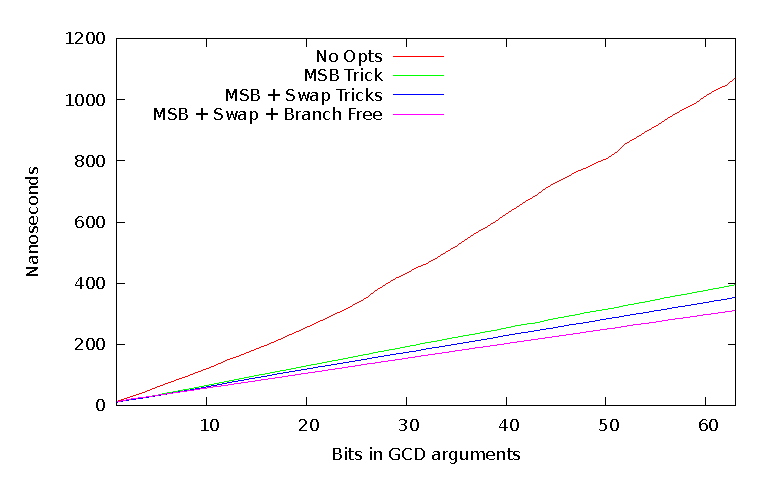
\includegraphics[scale=0.86]{xgcd-binary-optimizations-64}
\end{figure}
\end{frame}


% SQUARE ROOT APPROXIMATION
\begin{frame}
\frametitle{Approximate Square Root}
Notice that
\begin{equation*}
\begin{array}{rrlrlr}
	& x^{1/2} &=& 2^{(\log_2x)/2} &\approx& 2^{\floor{\floor{\log_2x+1}/2}} \\
	\Rightarrow & x / x^{1/2} &=& x / 2^{(\log_2x)/2} &\approx& x / 2^{\floor{\floor{\log_2x+1}/2}},
\end{array}
\end{equation*}
which is approximated by shifting $x$ right by $\floor{\floor{\log_2x+1}/2}$ bits.
\end{frame}

% SQRT OPTIMIZATION
\begin{frame}
\frametitle{Square Root Approximation}
\framesubtitle{64-bit ideal multiplication}
\begin{figure}
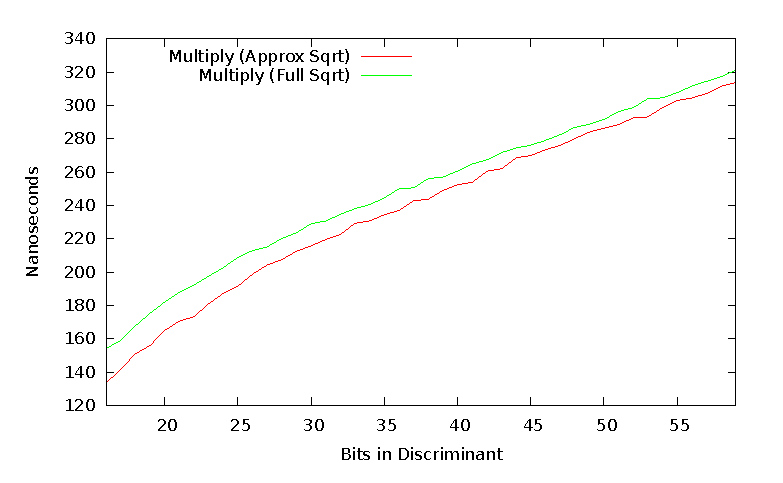
\includegraphics[scale=0.86]{compose-sqrtopt-64}
\end{figure}
\end{frame}

\begin{frame}
\frametitle{Square Root Approximation}
\framesubtitle{128-bit ideal multiplication}
\begin{figure}
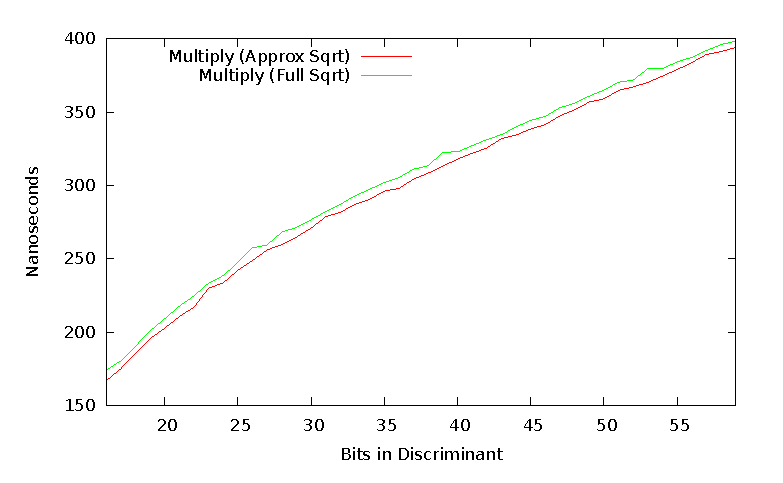
\includegraphics[scale=0.86]{compose-sqrtopt-128}
\end{figure}
\end{frame}

\begin{frame}
\frametitle{Square Root Approximation}
\framesubtitle{64-bit ideal cubing}
\begin{figure}
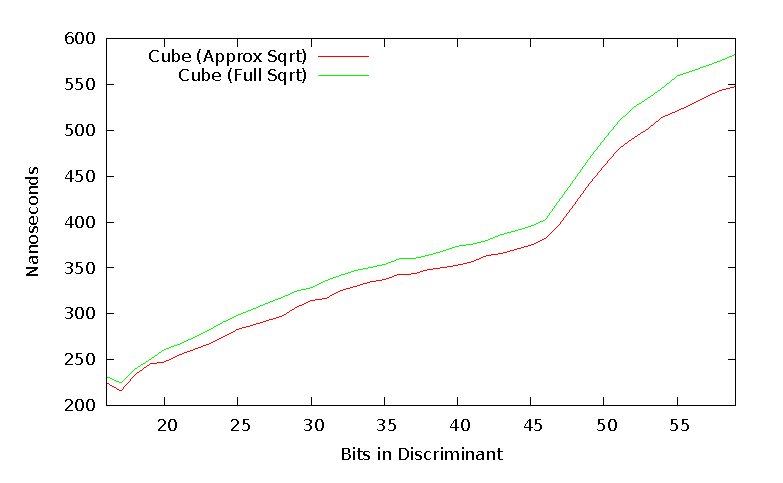
\includegraphics[scale=0.86]{cube-sqrtopt-64}
\end{figure}
\end{frame}

\begin{frame}
\frametitle{Square Root Approximation}
\framesubtitle{128-bit ideal cubing}
\begin{figure}
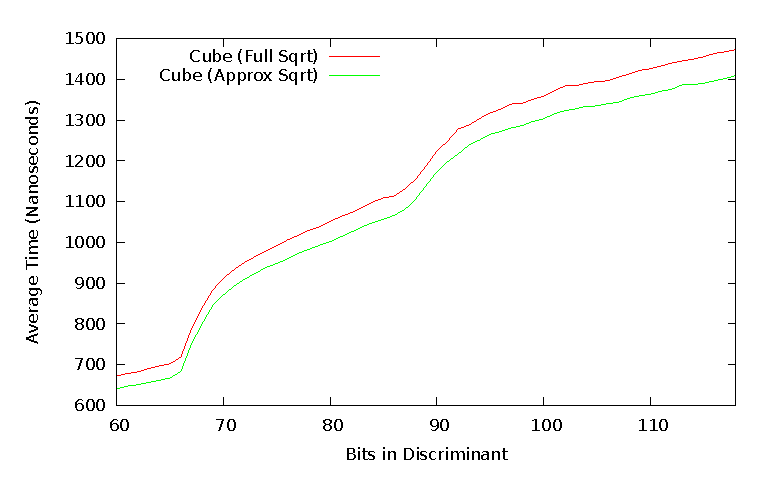
\includegraphics[scale=0.86]{cube-sqrtopt-128}
\end{figure}
\end{frame}

\begin{frame}
\frametitle{SuperSPAR Search Space}
\framesubtitle{48-bit semiprimes}
\begin{figure}
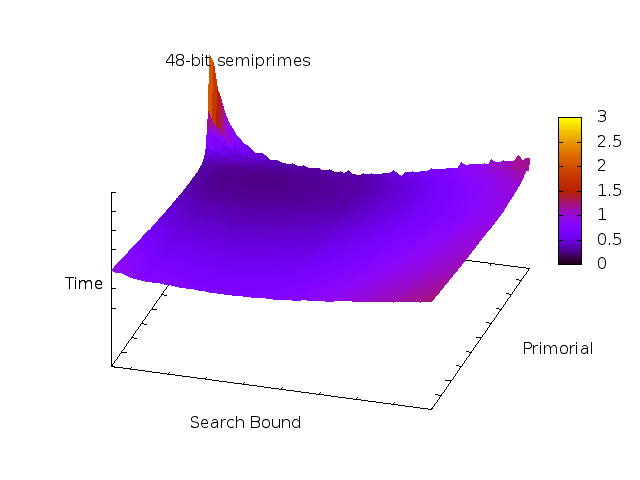
\includegraphics[scale=0.47]{bits-48-3d.png}
\end{figure}
\end{frame}
\begin{frame}
\frametitle{SuperSPAR Search Space}
\framesubtitle{56-bit semiprimes}
\begin{figure}
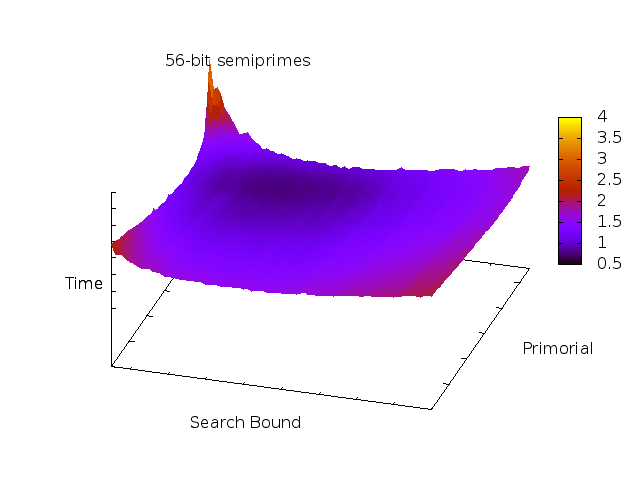
\includegraphics[scale=0.47]{bits-56-3d.png}
\end{figure}
\end{frame}
\begin{frame}
\frametitle{SuperSPAR Search Space}
\framesubtitle{64-bit semiprimes}
\begin{figure}
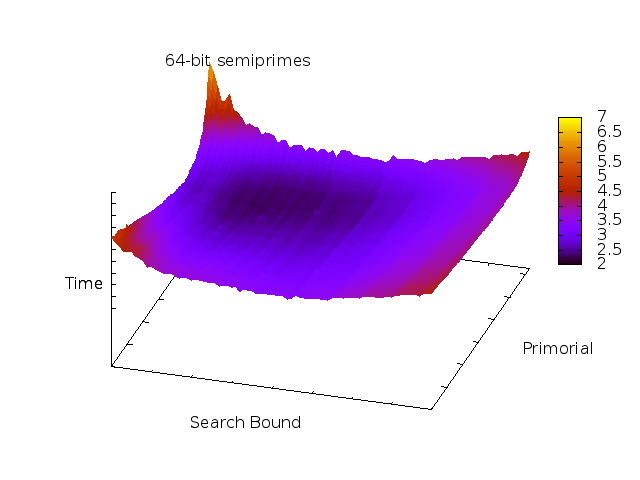
\includegraphics[scale=0.47]{bits-64-3d.png}
\end{figure}
\end{frame}
\begin{frame}
\frametitle{SuperSPAR Search Space}
\framesubtitle{72-bit semiprimes}
\begin{figure}
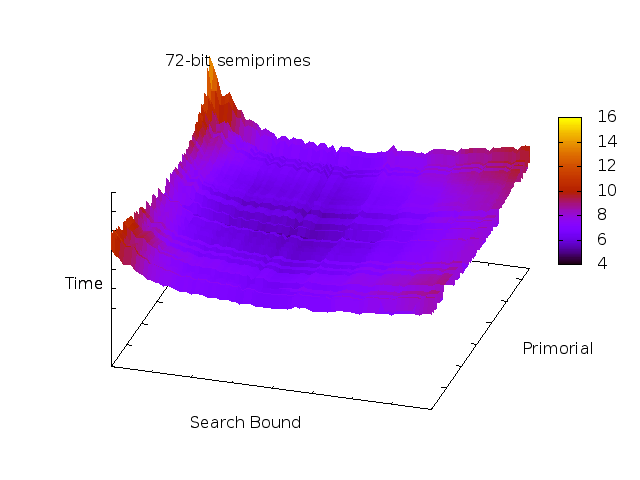
\includegraphics[scale=0.47]{bits-72-3d.png}
\end{figure}
\end{frame}
\begin{frame}
\frametitle{SuperSPAR Search Space}
\framesubtitle{80-bit semiprimes}
\begin{figure}
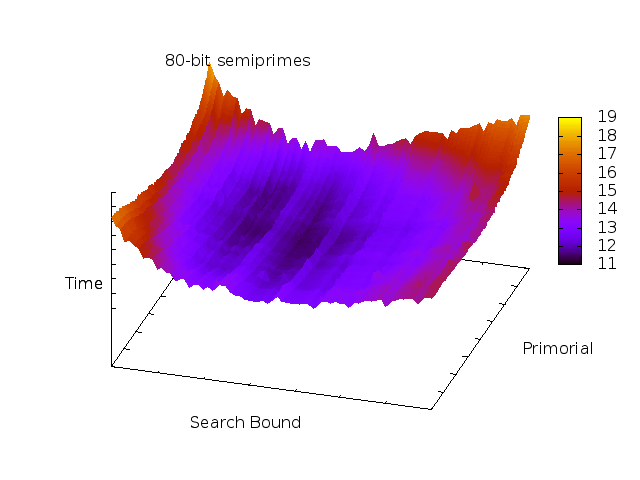
\includegraphics[scale=0.47]{bits-80-3d.png}
\end{figure}
\end{frame}

\begin{frame}
\frametitle{SuperSPAR Prime Ideals}
\framesubtitle{Sequential vs Random}
\begin{figure}
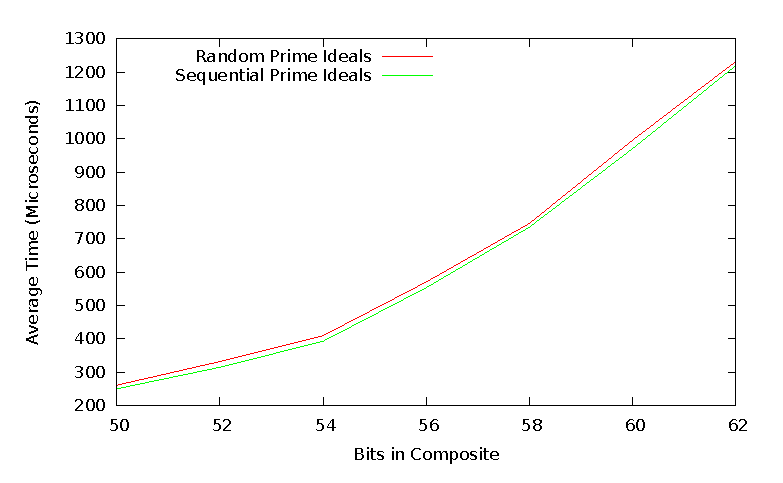
\includegraphics[scale=0.86]{sspar-random-vs-sequential}
\end{figure}
\end{frame}


\begin{frame}
\frametitle{SPAR -- Expanding the 2-Sylow Group}
\begin{table}
\centering
\begin{tabular}{| r | r | r |}
	\hline
	Bits & With 2-Sylow Group & Without 2-Sylow Group \\
	\hline
	16 &   48.05208 &   48.02160 \\
	20 &   84.20318 &   84.09526 \\
	24 &  197.02479 &  196.84587 \\
	28 &  463.70674 &  463.60538 \\
	32 &  937.57875 &  935.81785 \\
	36 & 1709.55629 & 1706.32960 \\
	40 & 3255.31447 & 3248.67998 \\
	\hline
\end{tabular}
\caption{Average time in microseconds to factor using SPAR when the number of ideals per class group is bound by the size of the integer to factor.}
\end{table}
\end{frame}

\begin{frame}
\frametitle{Simple Continued Fraction Expansion of $K / L$}
Recurrences:
\begin{align*}
R_i &= R_{i-2} - q_i R_{i-1} \\
C_i &= C_{i-2} - q_i C_{i-1} \\
A_i &= A_{i-2} + q_i A_{i-1} \\
B_i &= B_{i-2} + q_i B_{i-1}
\end{align*}

Invariants:
\begin{align*}
C_i &= (-1)^{i+1} B_i \\
L &= R_iB_{i-1} + B_iR_{i-1} \\
(-1)^{i-1} &= A_iB_{i-1} - B_iA_{i-1} \\
(-1)^{i+1} R_i &= LA_i - KB_i \\
\end{align*}
\end{frame}

\end{document}

